% -*- mode: fundamental -*-

% ****************************************************************

\chapter{RISC-V: Optimizing Drum and Fife}

\markboth{Ch \arabic{chapter}: RISC-V: Optimization}{\copyrightnotice}

\setcounter{page}{1}
% \renewcommand{\thepage}{\arabic{page}}
\renewcommand{\thepage}{\arabic{chapter}-\arabic{page}}

\label{ch_Optimization}

% ****************************************************************

\section{Introduction}

There are three physical dimensions on which we may want to optimize a
CPU design:

\begin{itemize}

 \item Time (performance): The speed (wall-clock time) at which a
       desired application is executed by the CPU.

 \item Space (area/resources): On ASICs, the silicon area occupied by
       the design.  For ASICS this may be measured in square
       millimeters or in ``number of gates''.  For FPGAs this may be
       measured in LUTs (Lookup Tables), BRAMs, DSPs and so on.
       Smaller is better, for many reasons (better silicon yields,
       lower power consumption, {\etc}.

 \item Energy: the amount of energy consumed to execute a desired
       application. Smaller is better.

\end{itemize}

These are not independent dimensions; improving one dimension often
costs something in another dimension.  Ultimately, a competitive
product specification for a particular target market will define the
acceptable boundaries for each dimension.

We will not say much in this book about energy optimization, even
though it is of course increasingly important in modern times, both in
the macro sense (reduce energy consumption for a greener planet) and
in the micro sense (mobile devices and IoT (Internet of Things)
devices work on battery power or energy harvested from the
environment).  Modern designs have many techniques to slow down or
switch off clocks, and reduce circuit-supply voltage for less critical
or idle circuits, both of which reduce energy consumption.

Regarding Performance, it is important to keep in mind that the
ultimate number that matters is \emph{application performance}, {\ie}
how long does it take to execute an application of interest. One will
often hear other numbers cited as, such as clock speed, instructions
per clock (IPC) or its inverse clocks per instruction (CPI), or total
number of instructions.  All these contribute to application
performance; they do not individually determine application
performance.  Conceptually, the total execution time for an
application is:

\begin{tabbing}
\hmmm \= <exec time> \= $=$ <total number of instrs> \hm \= $\times$ \= $1/$<clock-speed> \hm \= $\times$ \= CPI \\
\\
\hm the units being: \\
\\
      \> seconds     \> $=$ instructions                 \> $\times$ \> seconds/cycle         \> $\times$ \> cycles/instruction
\end{tabbing}

For a given application and a given set of input data, total number of
instructions is a function of the ISA and compiler quality.  ISAs like
x86 or the older DEC PDP-11, DEC Vax, and Motorola 68000 were
\emph{Complex Instruction Sets}, where a single ``CISC'' instruction
could express more work, such as a memory read, an integer op, and a
memory write.  RISC-V is a \emph{Reduced Instruction Set}, where that
same work needs separate ``RISC'' instructions for LOAD, Integer and
STORE.  And, of course, a better compiler may produce a smaller
program (fewer instructions) from the same source code.

CPI is not a constant.  First, it may vary inherently across different
kinds of instructions---an integer ALU instruction may take fewer
cycles than a memory-access instruction or a floating-point
instruction.  Second, even for a particular kind of instruction, CPI
may vary; for example, the number of cycles for a memory-access
instruction may depend on hits/misses in caches, hits/misses in
virtual memory TLBs (Trqnslation Lookaside Buffers), {\etc}.  Third,
an integer that reads a register may stall for a number of cycles
because a preceding instruction has not yet written the register.
Thus, in the above formula, CPI is just an average CPI across the
application.

Clock speed may not be constant; in some implementations, clocks are
slowed down, or even switched off for non-performance-critical
components during intervals that do not demand high performance ({\eg}
``idling'').

The terms in the formula above need simultaneously to be optimized for
the best product.  They are not independent; higher clock speeds
restrict how much ``circuit work'' can be done in a single clock
which, in turn, affects microarchitecture ({\eg} may need to split an
operation into multiple pipeline stages); which, in turn, can affect
instructions/cycle.  A CISC ISA may get more work done with fewer
instructions, but a RISC ISA may be implementable with much higher
clocks speeds and more pipeline parallelism.

Instructions/cycle depends on microarchitecture.  The more parallelism
we can exploit, the higher the instructions/cycles that can be
achieved.  A common term to refer to this measure is ``ILP''
(Instruction-Level Parallelism).

For example, in both Drum and Fife, any particular instruction takes
five or more cycles, from Fetch to Retire.  Drum, having an FSM
microarchitecture, therefore retires one instruction every five or
more cycles.  Fife, which executes many instructions in parallel in
its pipelined microarchitecture, can often retire one instruction per
cycle.

\index[RV]{superscalar microarchitecture}
\index[RV]{microarchitecture!superscalar}

An advanced microarchitecture with more parallelism is the
\emph{superscalar} microarchitecture, which may fetch and execute 2 or
4 (or more) instructions at a time.

\index[RV]{out-of-order microarchitecture}
\index[RV]{microarchitecture!out-of-order}

\index[RV]{cache!non-blocking}
\index[RV]{cache!hit-under-miss}

Another advanced microarchitecture with more parallelism is the
\emph{out-of-order} microarchitecture which may, for example, have
multiple integer execution units, and allow multiple integer
instructions to execute at a time, or even out-of-order depending on
when their input data is available.  The cache in their DMem may
support ``non-blocking caches'' or ``hits-under-misses'' {\ie} for two
memory accesses $a_1$ and $a_2$ that arrive in that order, it permits
$a_2$ to be serviced while $a_1$ may be awaiting a cache-refill due to
a cache-miss.

Superscalarity and Out-of-order microarchitectures are beyond the
scope of this book.  In the rest of this chapter we will discuss
improving the resources and performance of Drum and Fife.

% ****************************************************************

\section{Pipeline traces and visualization to analyze performance}

Before trying to optimize a CPU, we must first analyze and understand
the existing implementation thoroughly so that we can then identify
opportunities for improvement.

\index[RV]{Pipeline trace}

The first step is to produce a \emph{pipeline trace}, which has more
fine-grain detail than a mere \emph{instruction trace} (which only
records the trace of instructions retired).  We record, for every
instruction, its transit through \emph{each} stage of the FSM (Drum)
or pipeline (Fife).

For example, if we examine the Fife code for \verb|rule rl_Decode| we
see an invocation of a chain of functions:

{\small
\begin{Verbatim}[frame=single, label=src\_Fife/S2\_Decode.bsv]
      log_Decode (rg_flog, y, rsp_IMem);
\end{Verbatim}
}

$\longrightarrow$

{\small
\begin{Verbatim}[frame=single, label=src\_Common/Fn\_Decode.bsv]
   function Action log_Decode (File flog, Decode_to_RR y, Mem_Rsp rsp_IMem);
      ...
      ftrace (flog, y.inum, y.pc, y.instr, "D", $format(""));
      ...
\end{Verbatim}
}

$\longrightarrow$

{\small
\begin{Verbatim}[frame=single, label=src\_Common/Utils.bsv]
function Action ftrace (File         flog, ...)
         ...
	 $fdisplay (flog, "Trace %0d %0d %0h %0h %s", cur_cycle,
		    inum, pc, instr, label, adhoc);
\end{Verbatim}
}

This writes a line like this into the logfile produced by Drum and
Fife when they are simulated:

{\small
\begin{Verbatim}[frame=single, label=log.txt]
...
Trace 6 2 80000008 fe012e23 D
...
\end{Verbatim}
}

which records the fact that on clock tick 6 (cycle 6), the $2^{nd}$
instruction, whose PC is \verb|0x8000_0008|, and whose 32 bits are
\verb|0xfe01_2e23|, was processed in the Decode stage.  Similarly, we
write a trace item for every interesting microarchitectural event for
each instruction.

By studying this code, manually or with analysis software, we can get
an idea of exactly how many cycles each instruction takes, and where
we may be ``losing cycles'', if any.

This trace can also be processed and displayed in a ``pipeline
visualization'' tool.  If we take the pipeline trace \verb|log.txt|
produced by Drum or Fife, we can run it through the Python program
\verb|Log_to_CSV.py| provided with Drum and Fife:

{\small
\begin{Verbatim}[frame=single, label=log.txt]
  $ Tools/Log_to_CSV/Log_to_CSV.py  log.txt  0 100
\end{Verbatim}
}

This selects from instruction 0 through instruction 100 from the
pipeline trace file, and produces a file \verb|log.txt.csv| in the
standard ``comma-separated variables'' data input format that is
accepted by most spreadsheed programs (OpenOffce, Microsoft Excel, Mac
Numbers, Google Sheets).

Figure~\ref{Fig_PipeViz} shows the display, in the Mac Numbers
spreadsheet application, for the pipeline trace of up to the first few
instructions for the ``Hello World!'' C program running on Drum and
Fife, respectively:
\begin{figure}[htbp]
  \centerline{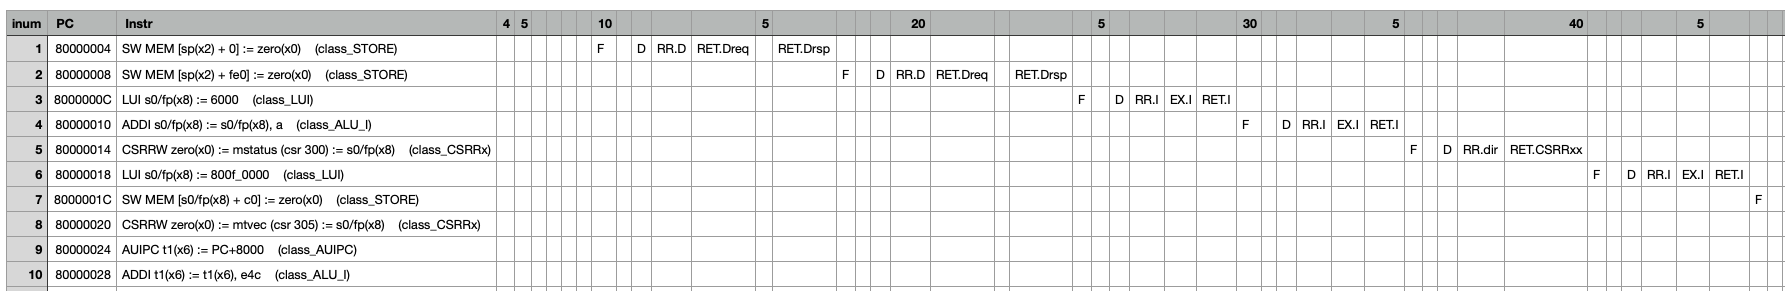
\includegraphics[width=6in,angle=0]{Figures/Fig_PipeViz_Drum}}
  \vspace*{1ex}
  \centerline{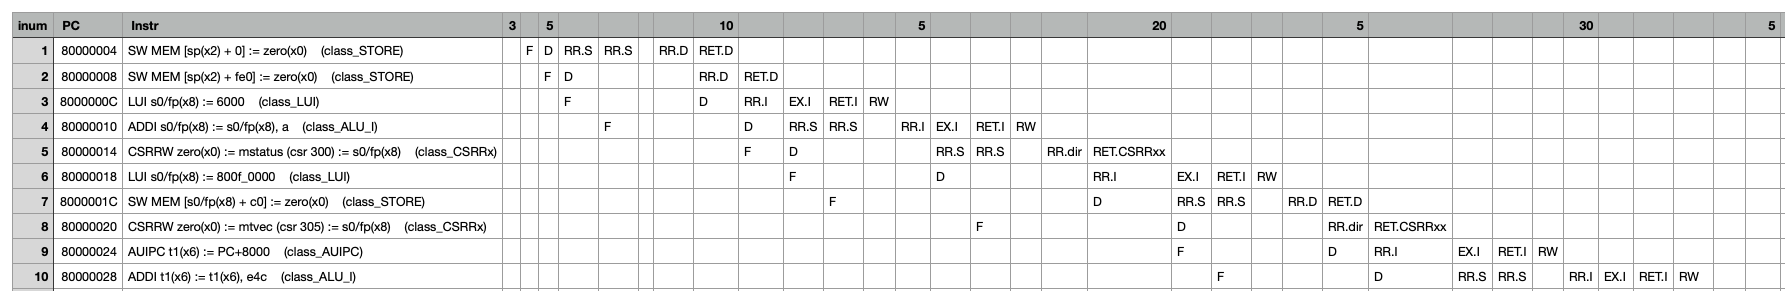
\includegraphics[width=6in,angle=0]{Figures/Fig_PipeViz_Fife}}
  \caption{\label{Fig_PipeViz}
           Visualization of the per-instruction stage events in Drum and Fife}
\end{figure}

In both displays, the vertical axis, going downwards, shows
instruction number 1, 2, 3, ...  The horizontal axis, going to the
right, shows the PC and disassembled instruction in the first two
columns, followed by clock ticks.  For each instruction, we see its
instruction numbrer, PC and dissassembly, and then the Drum/Fife stage
events at the clock tick where the event happened.

We can clearly see the difference between FSM sequenced (Drum) and
pipelined (Fife) behavior.  In Drum, after the first instruction has
completed (``RET.Drsp'' = Retire DMem Response) in tick 6, the Fetch
(``F'') for the second instruction occurs in tick 7.  In Fife, after
the Fetch for the first instruction on tick 4, the Fetch for the
second instruction occurs in tick 5, the very next tick.

Considering IPC, we can see that in Drum, we have barely completed 6
instructions at tick 46, whereas Fife is has finished 10 instruction
by tick 33.  The tradeoff, as suggested earlier, is that Drum takes
far fewer resouces (LUTs, gates) in silicon compared to Fife.

For each instruction, after its Fetch, horizontal gaps indicate lost
cycles, {\eg} an instruction stalling at Register Read because it is
waiting for an earlier instruction to write that register value, or a
memory access waiting for the memory response.  In Fife, we can also
see which instructions were discarded (more lost cycles) due to PC
misprediction or traps.

% ================================================================

\section{Optimization opportunities in Drum and Fife}

The following sections discuss a number for optimization opportunities
for Drum and Fife.  Whether they actually produce improvements or not
is usually difficult to predict just from observation or analysis,
because an optimization's improvement in one dimension may come at a
cost in another and, further, optimizations may interact positively or
negatively.  Ultimately, one must implement the optimizations and
\emph{measure} the actual impacts on clock speed, IPC, application
performance, resources, and energy consumption, {\etc} and then make a
deployment choice based on actual product priorities.

Each of these opportunties is a potential project for the reader of
this book, starting with the existing Drum or Fife code, for more
practice with RISC-V and BSV.  Almost all of them them require no new
BSV concepts beyond what has already been covered.

% ================================================================

\subsection{Drum and Fife: Fusing Decode and RR-Dispatch}

\label{Sec_Fuse_Decode_RR}

More FSM steps in Drum or more stages in Fife (longer pipelines) will,
in general, enable higher clock speeds (because the circuits in each
stage have less to do, and so have less circuit delay).  But more
stages increase the latency (number of ticks) for each instruction,
and the resources (more register or FIFO buffering between stages).

In some cases it is worthwhile going in the opposite direction, fusing
what used to be two stages into one.  A functionally easy pair to fuse
is Decode and RR-Dispatch.  In Drum, the Decode action looks like
this:

{\small
\begin{Verbatim}[frame=single, label=src\_Drum/CPU.bsv]
   Action a_Decode =
   action
      let mem_rsp <- pop_o (to_FIFOF_O (f_IMem_rsp));
      let y       <- fn_Decode (rg_Fetch_to_Decode, mem_rsp, rg_flog);
      rg_Decode_to_RR <= y;
      ...
   endaction;
\end{Verbatim}
}

It writes it output into the \verb|rg_Decode_to_RR| register.  The
Register-Read-and-Dispatch action looks like this and reads from the
register:

{\small
\begin{Verbatim}[frame=single, label=src\_Drum/CPU.bsv]
   Action a_Register_Read_and_Dispatch =
   action
      let x       = rg_Decode_to_RR;
      ...
   endaction
\end{Verbatim}
}

We can fuse these into a single action, like this:

{\small
\begin{Verbatim}[frame=single]
   Action a_Decode_and_Register_Read_and_Dispatch =
   action
      // Decode part
      let mem_rsp <- pop_o (to_FIFOF_O (f_IMem_rsp));
      let y       <- fn_Decode (rg_Fetch_to_Decode, mem_rsp, rg_flog);
      // RR-and-dispatch part
      let x       = y;
      ...
   endaction
\end{Verbatim}
}

directly passing the output of Decode (\verb|y|) as \verb|x| in
Register-Read-and-Dispatch.  This allows us to eliminate the
\verb|rg_Decode_to_RR| register.  In the main Drum FSM, we replace the
original two sequenced actions:

{\small
\begin{Verbatim}[frame=single]
      a_Decode;
      a_Register_Read_and_Dispatch;
\end{Verbatim}
}

with a single action:

{\small
\begin{Verbatim}[frame=single]
      a_Decode_and_Register_Read_and_Dispatch;
\end{Verbatim}
}

The same fusion can be done in Fife as well: we fuse \verb|rl_Decode|
(in package \verb|S2_Decode|) with \verb|rl_RR_Dispatch| (in package
\verb|S3_RR_RW|) into a single rule, and eliminate the FIFOs
connecting the two modules (through which we were passing the
\verb|Decode_to_RR| intermediate value).

In both cases, we reduce, by 1 tick, the transit through Decode and
Register-Read-and-Dispatch, and we eliminate the intermediate buffer
(register or FIFOs), both of which appear to be improvements.

On the other hand, the depth of the combined stage combinational
circuit is now the sum of the depths in the original two stages; this
may reduce the clock speed at which we can run it.

\index[RV]{Pipeline!balanced and unbalanced}
\index[RV]{Pipeline!slack}
\index[RV]{Timing!slack}

Fusion may not reduce the achievable clock speed if some other stage
already limits the achievable speed.  In this case we would say that
the pipeline was originally ``unbalanced'' and that fusion has brought
it closer to balance (all stages having approximately the same
combinational delay).  Fusion has merely utilized some timing
``slack'' that was already available in the two stages.

% ================================================================

\subsection{Drum and Fife: Fusing some Retire actions}

In both Drum and Fife, exception handling is done by itself in a
separate rule.  In Drum, it is the last, separate action in the FSM,
\verb|a_exception|, in module \verb|mkCPU| in \verb|src_Drum/CPU.bsv|.
In Fife, it is in rule \verb|rl_exception| in module module
\verb|mkRetire| in \verb|src_Fife/S5_Retire.bsv|.

In both cases, the exception is actually detected in earlier rules,
which save values in three registers \verb|rg_epc|, \verb|rg_cause|
and \verb|rg_tval| which are then used by the exception handling
action.

Similar to the fusion idea of Section~\ref{Sec_Fuse_Decode_RR}, the
exception-handling action can be fused directly into the earlier
actions where the exception was detected, and the three registers can
be eliminated.

This transformation to reduce ticks for exception-handling may be less
important because, almost by definition, exceptions should be rare,
and therefore saving this tick may not affect application performance
very much.

% ================================================================

\subsection{Drum (rules version): short-circuiting stages}

In the ``rules'' version of Drum (\verb|src_Drum/Drum_Rules.bsv| and
described in Chapter~\ref{ch_Drum_Rules}), the ``retire'' rules
(\verb|rl_Retire_direct|, \verb|rl_Retire_Control|
\verb|rl_Retire_Int| and \verb|rl_Retire_DMem| set the next action to
\verb|A_EXCEPTION|.

This, in turn, enables the next rule \verb|rl_exception| which tests
whether there actually was an exception, and if not, sets the next
action to \verb|A_FETCH|.

This structure emerged due to a blind mechanical mimicing of the
structure of the \verb|StmtFSM| version of Drum.

Instead, in each of the ``retire'' rules, we can replace:

{\small
\begin{Verbatim}[frame=single]
      rg_action <= A_EXCEPTION;
\end{Verbatim}
}

with:

{\small
\begin{Verbatim}[frame=single]
      rg_action <= (rg_exception ? A_EXCEPTION : A_FETCH);
\end{Verbatim}
}

allowing it to ``jump'' back to FETCH immediately, instead of spending
another tick in rule \verb|rl_exception|.

This kind of ``jump'' is not possible in \verb|StmtFSM|, which only
allows structured compositions of sequencing and if-then-else.

% ================================================================

\subsection{Drum: using narrower inter-stage buffers}

Consider the output of the \verb|fn_Dispatch| in
\verb|src_Common/Fn_Dispatch.bsv|, with the following type:

\input{Code_Extracts/Result_Dispatch}

In Drum, this result is stored in register \verb|rg_Dispatch|.  The
width of this buffer is the sum of the widths of each of the four
component types:

\begin{tabbing}
\hmm \= \hmm \= Number of bits in {\tt to\_Retire} \\
     \> $+$  \> Number of bits in {\tt to\_EX\_Control} \\
     \> $+$  \> Number of bits in {\tt to\_EX} \\
     \> $+$  \> Number of bits in {\tt to\_EX\_DMem}
\end{tabbing}

The \verb|to_Retire| field has type \verb|RR_to_Retire|, which
contains an \verb|exec_tag| field, whose type is:

\input{Code_Extracts/Exec_Tag}

Observe that \verb|exec_tag| determines which of fields in the result
of \verb|fn_Dispatch| other than \verb|to_Retire| are relevant:

\begin{tightlist}

 \item When \verb|exec_tag| is \verb|XEC_TAG_CONTROL| then
       only the \verb|to_EX_Control| field is relevant.

 \item When \verb|exec_tag| is \verb|XEC_TAG_INT| then
       only the \verb|to_EX| field is relevant.

 \item When \verb|exec_tag| is \verb|XEC_TAG_DMEM| then
       only the \verb|to_EX_DMem| field is relevant.

\end{tightlist}

With this observation, we can see that, in \verb|rg_Dispatch|, we can
have a common set of bits shared by these three cases.  Then, the
number of bits in \verb|rg_Dispatch| could be reduced to:

\begin{tabbing}
\hmm \= \hmm \= Number of bits in {\tt to\_Retire} \\
     \> $+$  \> max ( \= Number of bits in {\tt to\_EX\_Control} \\
     \>      \>       \> Number of bits in {\tt to\_EX} \\
     \>      \>       \> Number of bits in {\tt to\_EX\_DMem} )
\end{tabbing}

BSV has a convenient type-notation to express this ``overlaying of
alternatives''.  In this case, it would look like this:

{\small
\begin{Verbatim}[frame=single]
typedef struct {
   RR_to_Retire      to_Retire;    // without the exec_tag field

   union tagged {
      void              EXEC_TAG_DIRECT;
      RR_to_EX_Control  EXEC_TAG_CONTROL;
      RR_to_EX          EXEC_TAG_INT,
      Mem_Req           EXEC_TAG_DMEM
   } exec_tag

} Result_Dispatch
deriving (Bits, FShow);
\end{Verbatim}
}

The new nested \verb|exec_tag| field combines the previous ``enum''
type and the 3 struct fields into a single ``union'' indicating the
alternatives for each tag.

% ================================================================

\subsection{Fife: saving FIFO resources}

In Section~\ref{Sec_Fife_connections} with
Figure~\ref{Fig_Fife_connections} and in
Section~\ref{Sec_mkBypassFIFOF_mkPipelineFIFOF} with
Figure~\ref{Fig_Composed_FIFO_modularity} we described how we connect
Fife stages in a modular way, using a pair of FIFOs---a BypassFIFO in
one stage (module) and a PipelineFIFO in the other, connected using
\verb|mkConnection| in the parent CPU module.  We also explained how,
while improving modularity, separate compilation and stage
independence, it also costs us in resources: inside the pair of FIFOs
are two data registers for what is essentially used as a 1-element
FIFO.

We may now selectively optimize these FIFO pairs, replacing such a
pair by a single FIFO. The upside is that the buffer now has just one
register for the buffer.  The downsides are (a) we now have a
scheduling constraint across the buffer, where the rule on one side
has to be scheduled before the rule on the other side, and (b) we now
have a combinational path spanning both both stages.  The longer
combinational path may reduce achievable clock speed.

Whether we use a PipelineFIFO or a BypassFIFO for this purpose depends
on where it is used, because of the scheduling constraint.  Usually we
will need a PipelineFIFO in a forward path and a BypassFIFO in a
reverse path because, for pipeline behavior we need to schedule a
downstream rule before an upstream rule.

% ================================================================

\subsection{Fife: Reducing the misprediction penalty}

\label{Sec_misprediction_penalty}

In Fife, in Fetch stage, after issuing an IMem read-request for the
instruction using the address in \verb|rg_pc|, it ``predicts'' the
next instruction address to be \verb|rg_pc+4|.  That prediction could
of course be wrong, if the previous instruction is a BRANCH or JUMP
that takes it somewhere else, or if it traps, which takes it to the
instruction address of the trap-handling code.

As described in Section~\ref{Sec_Epochs}, we manage these
``mispredictions'' using ``epochs''.  At any given time, we are in
some particular prediction epoch.  In Fetch, we attach the current
epoch and the current next-instruction prediction to the
instruction. In Retire, we can definitively check the next-instruction
prediction.  If mispredicted, we increment the epoch redirect Fetch
with the correct PC and new epoch.  Retire starts discarding all
subsequent instructions thqt have the old epoch, because they are all
in the ``misprediction shadow'', and resumes normal operation only it
sees the first instruction carrying the new epoch.

\index[RV]{misprediction!penalty}
\index[RV]{misprediction!shadow}
\index[RV]{misprediction!manage with epochs}
\index[RV]{PC-prediction!misprediction}

The time wasted on these discarded instructions is called the
``\emph{misprediction penalty}''.  Clearly, we would like to reduce
this wasted time.

% ----------------------------------------------------------------

\subsubsection{Save a tick for Fetch redirection using CRegs}

In package \verb|S1_Fetch|, rule \verb|rl_Fetch_req| reads
\verb|rg_pc| for the instruction address used for IMem requests, and
reads \verb|rg_epoch| to accompany the instruction down the pipe (A).

Concurrently, \verb|rl_Fetch_from_Retire| updates \verb|rg_pc| and
\verb|rg_epoch |with a redirected PC and new epoch (B).

When \verb|rg_pc| is a standard register, the update from (B) is
visible to (A) only on the next tick.

Suppose:
\begin{tightlist}

 \item we replace \verb|rg_pc| and \verb|rg_epoch| by CRegs \verb|crg_pc|
       and \verb|crg_epoch| ((Section~\ref{Sec_CRegs});

 \item we replace the register-writes (B) with a writes to \verb|crg_pc[0]|
       and \verb|crg_epoch[0]|, and

 \item we replace the register-reads (A) with reads from
       \verb|crg_pc[1]| and \verb|crg_epoch[1]|.

\end{tightlist}
Then, the updates in (B) is visible to (A) in the \emph{same} tick.

Caution: we now have combinational paths (through the CReg) from
(B) into (A), with a potential negative impact on clock speed.

% ----------------------------------------------------------------

\subsubsection{Save a tick for Fetch redirection by eliminating backward FIFO}

Currently, the redirection from Retire back to Fetch spends a tick in
a FIFO (see FIFOs \verb|f_Fetch_from_Retire| in Retire and in Fetch
stages).

We can eliminate this tick by having Retire directly write into
registers \verb|rg_pc| and \verb|rg_epoch| for the redirection update.

Caution: we have reduced the isolation of the two stages Retire and
Fetch, resulting in longer combinational paths, with a potential
negative impact on clock speed.

% ----------------------------------------------------------------

\subsubsection{Quicker reaction to redirection by Register-Read and Dispatch}

Currently, mispredicted instructions go through all their usual
processing before being discarded at Retire.  This may include several
delays and possibly use resources:

\begin{tightlist}
 \item Stall at Register-Read due to read/write hazards.

 \item Reserve an Rd register, which then has to be un-reserved by
       Retire when the instruction is discarded.

 \item Spend multiple cycles in some execution stages (memory-access,
       integer multiply/divide, floating-point, ...).

 \item For DMem ops, ``pollute'' the cache with unnecessary accesses 

 \item For DMem STORE ops, use up an entry in the store-buffer which
       then has to be discarded by Retire when the instruction is
       discarded.

\end{tightlist}

If, in addition to the Retire$\longrightarrow$Fetch redirection
message, we also feed the message to the Decode stage and/or the
Register-Read-and-Dispatch stage, they can immediately start
discarding wrong-epoch instructions, or convert them into no-ops.  In
either case, they no longer encounter the delays or use resources as
listed above.

% ----------------------------------------------------------------

\subsubsection{Better next-PC prediction}

\label{Sec_better_next_PC_prediction}

The Fetch stage currently performs a fixed next-PC prediction like this:

{\small
\begin{Verbatim}[frame=single, label=src\_Fife/S1\_Fetch.bsv]
      let pred_pc = rg_pc + 4;
\end{Verbatim}
}

This is not bad, since in most codes there are medium to long
stretches of ``straight-line'' code between BRANCH and JUMP
instructions.  Applications in the ``scientific'' domain have a lot of
well-structured loops operating on vectors and rectangular matrices;
in these applications it is often possibly to ``unroll'' loops
significantly, producing \emph{very} long sequences of straight-line
code (hundreds of instructions).

Still, prediction can be improved further; in modern processors,
prediction success rates can be in the high 90\% range, close to
100\%.

Let us restructure the code slightly.  Suppose, in this module
\verb|mkFetch|, we have instantiated a ``\verb|pc_predictor|'' module
with a ``\verb|pc_predict|'' ActionValue method

{\small
\begin{Verbatim}[frame=single, label=src\_Fife/S1\_Fetch.bsv]
      let pred_pc <- pc_predictor.predict (rg_pc);
\end{Verbatim}
}

If the \verb|pc_predict| method simply increments its argument by 4
and returns it, we are at status quo, {\ie} equivalent to the original
code.  But now we can replace the \verb|pc_predictor| module with more
sophisticated versions for better prediction.

% ----------------

\paragraph{Branch Target Buffers}

\label{Sec_BTBs}

\index[RV]{PC prediction!BTBs (Branch Target Buffers)}

One technique is to add a ``\emph{Branch-Target Buffer}'' (BTB), which
is a table associating the PC of a BRANCH instructions with the
next-PC when the BRANCH was recently executed.

Consider a simple loop like this:

\begin{tabbing}
\hmm \= B2: \hm \= \kill
     \>         \> initialize loop index and limit \\
     \> B1:     \> conditional BRANCH to B3 if loop index > limit \\
     \>         \> ... \\
     \>         \> loop body and increment loop index \\
     \>         \> ... \\
     \> B2:     \> unconditional BRANCH to B1 \\
     \> B3:
\end{tabbing}

Suppose the loop iterates 100 times. Our simple PC+4 prediction will
fail on every loop iteration at B2, and once at B1 at the end of the
loop, {\ie} there will be 101 mispredictions.

When the branch at B1 or B2 reaches Retire, we know whether it was
mispredicted or not.  If mispredicted, then in the redirection message
sent back to Fetch, we also indicate that this was a BRANCH
instruction. In Fetch, in rule \verb|rl_Fetch_from_Retire| where we
update the PC and epoch, we also invoke a method \verb|branch_train()|
in the \verb|pc_predictor| module informing it about the BRANCH's PC
and the actual next-PC, and this pair is stored in the BTB table.

In the \verb|pc_predict(pc)| method, we consult the BTB for the
argument PC.  If we find a match, we return the associated next-PC;
else, we return the default PC+4 prediction.

Now let us consider again our loop example.  The first time we arrive
at B2 we will mispredict PC+4, because B2 is not yet in the BTB, but
we will also enter (B2,B1) into the BTB.  In subsequent arrivals at
B2, we will find B2 in the BTB and correctly predict that the next-PC
is B1.  Regarding B1, for the first 100 arrivals we will predict PC+4
(the default prediction) which is correct, but at the 101st (last)
arrival this will be a misprediction.

The net outcome is that for the whole loop, where previously we had
101 mispredictions, the BTB reduces it to just 2 mispredictions.  Also
remember that ``101'' was based on the number of loop iterations (we
assumed 100)---for a 1000-iteration loop, we would have 1001
mispredictions.  The simple BTB has reduced it to a constant 2
mispredictions, no matter how many iterations.

% ----------------

\paragraph{Adding hysteresis to the BTB}

\label{Sec_BTBs_w_hysteresis}

\index[RV]{PC prediction!BTB with hysteresis}

Consider executing our example loop a second time (perhaps it is
nested inside an outer loop, or is in a function that has been called
twice).  Now, B2 will have no mispredictions, because the BTB already
has a (B2,B1) entry.  The first time we encounter B1 it will be
mispredicted, because the last time we executed the loop, at loop exit
we would have entered (B1,B3) into the BTB, whereas now we need PC+4.
This misprediction will restore B1's prediction back to PC+4, and so
for subsequent iterations, B1 will predict correctly. On the last
iteration, B1 will again mispredict as PC+4, instead of B3.  Thus, we
have two mispredictions for the loop.

One technique is to add a little ``hysteresis'' or ``delay''into the
BTB.  From Retire, we were sending a redirection message back to Fetch
only on mispredictions.  Now, suppose Retire \emph{always} sends a
message to Fetch for BRANCH instructions; in the case of a correct
prediction, this is not a redirection but merely a confirmation of
correct prediction.  For each entry in the BTB, suppose we associate a
1-bit counter.  When we create a new entry in the BTB, we enter
(pc1,pc2,0).  When we subsequently receive a confirmation for this
prediction, we increment it to (pc1,pc2,1).  The first time we receive
a misprediction/redirection for pc1, we decrement it to (pc1,pc2,0),
{\ie} we don't change the BTB prediction, we merely reduce the
``confidence level'' of the prediction.  The second time we receive a
misprediction/redirection for pc1, we change the prediction to the
redirected pc.  Thus the 1-bit counter ``delays'' the change in the
BTB.

Now consder again our example loop.  In the first execution of the
loop (with no entry for B1 in the BTB), from the first iteration we
get (B1,B1+4,0) in the BTB, and from the second iteration onwards we
have (B1,B1+4,1). After the 100th iteration, B1 will mispredict (it
branches to B3).  The BTB entry will decrement to (B1,B1+4,0), but we
do not change the prediction.  Now, in the second execution of the
loop, in the first interation, we will predict correctly, with the BTB
entry now incrementing again to (B1,B1+4,1).  We will mispredict only
after the final iteration, on the loop exit.  Thus, in repeated
executions of this loop, we have reduced the mispredictions from 2 to
1.  If this loop is executed 1000 times (it is nested inside another
loop), that reduction of mispredictions goes from 2000 to 1000.

% ----------------

\paragraph{Control-flow-indexed BTBs}

\label{Sec_BTBs_w_cf_index}

\index[RV]{PC prediction!BTB, control-flow-indexed}

In many RISC-V programs we will find that we can more accurately
predict the outcome of a BRANCH if we knew how we arrived at that
BRANCH, {\ie} the instruction trace that preceded that BRANCH.  We
don't need every instruction in the preceding trace, just a trace of
recent BRANCHes, {\ie} something that summarizes the \emph{control
flow} leading up to the BRANCH.  Some BTBs are indexed by a short
control-flow trace ending at the BRANCH PC, instead of just the BRANCH
PC by itself.

% ----------------

\paragraph{Return Address Stacks}

\label{Sec_RAS}

\index[RV]{PC prediction!RAS (Return Address Stack)}

JAL instructions are mostly used for subroutine calls, and JALR
insructions are mostly used for subroutine returns (also subroutine
calls to ``distant'' addreses or computed addresses) .  By convention,
compilers use RISC-V register \verb|x1| (also known as \verb|ra|) for
the saved ``return address'' (saved in a call and used in a return).
Thus, when we see a JAL or JALR whose Rd register field is \verb|x1|,
it is probably a subroutine call.  When we see a JALR instruction
whose \verb|rs1| field is \verb|x1| and whose 12-bit immediate field
is 0, it is probably a subroutine return.  These observations (that a
JAL or JALR is likely a call or return) can detected in the Decode
stage; when the instruction reaches Retire, it can pass this
information to Fetch on the redirect path, and there it can be
recorded in the PC predictor sub-module.

In the PC predictor module, we can maintain a small local stack called
the ``Return Address Stack'') or RAS.  When asked to predict for a PC
that is known to be a subroutine call, in addition to the prediction
we can push PC+4 on the RAS.  When asked to predict for a PC that is
known to be a subroutine return, we can pop the prediction from the
RAS.  In effect, the RAS is ``shadowing'' or ``mimicing'' what happens
on the actual program stack for return-addresses.

% ----------------

\paragraph{Final remarks on PC prediction}

The PC-predictor module requires careful engineering.  First, the
\verb|pc_predict| method must be fast---it is invoked on every cycle
by \verb|rl_Fetch| in the Fetch stage.  Thus, BTBs and RASs cannot be
too large, otherwise it will not be possible perform lookups at speed.
Updates to the BTB and RAS (due to fresh information from Retire) must
occur concurrently with lookups, but not interfere with lookups.

There is also a potential security problem with PC predictors.  PC
predictors, in their BTBs and RASs, are recording some abtracted
information about the behavior of a program.  Suppose we switch to
another (malicious) process without clearing this information. That
progam may be able to execute code that measures whether certain
branches are predicted or not, and thereby glean some information
about the orignal progam.  These kinds of ``side-channel'' attacks
have become quite famous in recent years.  One solution is to clear
the PC predictor state completely on a process-switch.  Another is to
partition the PC predictor state and to reserve and use different
partitions for different processes.

In general next-PC prediction can be viewed as an ``online
machine-learning'' problem.  It is a ``machine-learning'' problem
because we are ``training'' the PC predictor with a data set (past
trace of the program), and then we are making predictions based on
that training.  It is ``online'' because training is interleaved with
use (as opposed to ``offline'', where training and use are completely
separate phases).  It is also ``online'' because training is happening
on live data, not a previously collected data set.  These observations
suggest some ideas for exploration:

\begin{itemize}

 \item Training does not have to be online.  One can run a program on
       a simulator and save precise prediction data to be pre-loaded
       into the online predictor.  This could be done on a shorter run
       of the program (smaller input data) if the prediction data
       remains stable.

 \item Modern machine-learning techniques could be applied to the
       prediction problem.

\end{itemize}

% ================================================================

\subsection{Fife: Reducing the register-hazard penalty}

\label{Sec_Reducing_Hazards}

The register-hazard penalty is the number of cycles an instruction I2
may stall (idle wait) in the Register-Read stage because one or more
of its input or output registers are ``busy''---there is an earlier
instruction I1 ahead of it in the pipeline that will be writing to one
of those registers.  This ``stall'' situation is detected and managed
using the scoreboard (Section~\ref{Sec_Scoreboards}).

% ----------------------------------------------------------------

\subsubsection{Fife Bypassing: Save a tick in GPRs and Scoreboard using CRegs}

In package \verb|S3_RR_RW|, rule \verb|rl_RR_Dispatch| reads
\verb|rg_scoreboard| to detect whether it should stall, and
\verb|gprs| when it can proceed (A).

Concurrently, \verb|rl_RW_from_Retire| updates \verb|rg_scoreboard|
and \verb|gprs| with new information from Retire (B).

When \verb|rg_scoreboard| is a standard register, and \verb|gprs| do
ordinary reads/writes into its underlying \verb|RegFile|, the updates
from (B) is visible to (A) only on the next tick.

Suppose we replace \verb|rg_scoreboard| with a 2-port CReg
\verb|crg_scoreboard| (Section~\ref{Sec_CRegs}). In
\verb|rl_RW_from_Retire| we write port [0] of the scoreboard, and in
\verb|rl_RR_Dispatch| we read port [1] of the scoreboard.  Then,
reading the scoreboard (A) can receive the updated value from (B) in
the same cycle.

We need to do something similar for the GPRs.  In module \verb|mkGPRs|
we add a 2-port CReg:

{\small
\begin{Verbatim}[frame=single, label=src\_Common/GPRs.bsv]
 Array #(Reg #(Tuple2 #(Bit #(5), Bit #(xlen)))) crg <- mkCReg (2, tuple2 (0, 0));
\end{Verbatim}
}

and we modify the methods as follows:

{\small
\begin{Verbatim}[frame=single, label=src\_Common/GPRs.bsv]
   method Bit #(xlen) read_rs1  (Bit #(5) rs1);
      match { .rd, .rd_val } = crg [1];
      return ((rs1 == rd) ? rd_val : regfile.sub (rs1));
   endmethod

   ... similarly read_rs2 ...

   method Action write_rd (Bit #(5) rd, Bit #(xlen) rd_val);
      let v = ((rd == 0) ? 0 : rd_val);
      crg [0] <= tuple2 (rd, rd_val);
   endmethod
\end{Verbatim}
}

Thus, when \verb|write_rd| and \verb|read_rd| are invoked in the same
cycle on the same register (\verb|rd| and \verb|rs1|, respectively),
the write-value \verb|rd_val| is passed directly to the read-method in
the same cycle (otherwise the read method gets it from the register
file, as usual).

With these two changes, we save one tick in the register-hazard delay.

Caution: we now have combinational paths (through the CRegs) from
(B) into (A), with a potential negative impact on clock speed.

% ----------------------------------------------------------------

\subsubsection{Fife: Dispatching multiple instructions that write to the same Rd}

Suppose we have two instructions, I1 followed by I2, that both write
to the same register Rd.  In the current code, I1 reserves Rd in the
scoreboard, and I2 stalls if I1 has not released the reservation (not
yet performed its write into the GPRs).  But I2 does not need the
value written to the GPR; so why did we stall?  Suppose there is a
third insruction I3 whose Rs1 == Rd.  If we had allowed I2 to proceed,
then when I1 finishes, it will release the Rd reservation, which will
allow I3 to proceed.  But this is wrong---I3 needs to wait for I2 to
write a value into the register, not take II's value.

Conceptually, we can think of the reservation bit for a register as a
1-bit counter indicating how many instructions (0 or 1) downstream
expect to write Rd.  We can generalize this idea. If we use 2 bits for
the reservation in the scoreboard, we can allow 0 to 3 instructions
downstream that expect to write Rd.  For I2, instead of stalling if
the reservation bit is 1, we now stall if the reservation bits value
is 3.  If the reservation bits value is $< 3$, we increment them and
allow I2 to proceed, {\ie} we have eliminated a stalling cycle.  When
I1 and I2 retire, we decrement the reservation bits.  For I3, we stall
until the reservation bits value is non-zero.

% ----------------------------------------------------------------

\subsubsection{Save a tick for register update by eliminating backward FIFO}

Currently, the register update from Retire back to
Register-Read-and-Dispatch spends a tick in a FIFO (see FIFOs
\verb|f_RW_from_Retire| in Retire and in Register-Read-and-Dispatch
stages).

We can eliminate this tick by having Retire directly write into
registers \verb|rg_scoreboard| and \verb|gprs|.

Caution: we have reduced the isolation of the two stages Retire and
Register-Read-and-Dispatch, resulting in longer combinational paths,
with a potential negative impact on clock speed.

% ================================================================

\subsection{Drum and Fife: Reducing memory system delays}

Memory systems are outside the scope of this book; this section is
mostly informational, to familiarize the reader with memory features
of interest.  We recommend \cite{Hennessy2017} for a more thorough
discussion of these topics.

A pipelined memory is one where the path through the memory system can
itself sustain one memory request per tick.  This allows the CPU
independently to pump in several memory requests into the memory
request channel, while concurrently pumping out memory responses for
previous requests from the memory response channel.  Ideally, the
memory system has a \emph{throughput} or \emph{bandwidth} of one
request per tick.

Memory \emph{latency} is the delay from when the CPU issues an IMem or
DMem request until it receives the corresponding IMem or DMem
response.

% ----------------------------------------------------------------

\subsubsection{TCMs (Tightly Coupled Memories)}

\index[RV]{SRAM (static RAM)}
\index[RV]{Memory!SRAM (static RAM)}

\index[RV]{Memory!BRAM (Block RAMs in FPGAs, which are SRAMs)}
\index[RV]{BRAM (Block RAMs in FPGAs, which are SRAMs)}

\index[RV]{TCM (tightly coupled memory)}

Small computer systems (embedded, IoT) often use a small TCM
(``Tightly Coupled Memory'') for their memory system.  TCMs are
usually implemented in SRAM (static RAM, BRAMs in FPGAs) which can be
accessed in 1 tick, so in these memory systems it is fairly
straightforward to have a 1-tick latench and also sustain a
1-request-per-tick throughput.

% ----------------------------------------------------------------

\subsubsection{Caches}

\index[RV]{DRAM (dynamic RAM)}
\index[RV]{Memory!DRAM (dynamic RAM)}

\index[RV]{Memory!Cache}
\index[RV]{Cache}
\index[RV]{Cache!miss penalty}

However, most modern systems have large memories based on DRAM
(Dynamic RAM), which can take many cycles to access both because DRAMs
are slower than SRAMs, and because requests and responses may have to
traverse many layers of interconnect between the CPU and the DRAM.  To
alleviate this delay, most systems use \emph{caches} close to the CPU.
Caches are often implemented in SRAMs so that, when a request ``hits''
in the cache ({\ie} the addressed word is already in the cache), it is
usually possible to perform the access in 1 tick.  On a cache
``miss'', on the other hand, the cache system has to ``refill'' the
missing data by fetching it from DRAM, and this can take many cycles.
The delay incurred here is called the ``cache miss penalty''.

\index[RV]{Memory!Cache!non-blocking}
\index[RV]{Cache!non-blocking}

Non-blocking caches are able to process another memory request R2
while it is servicing a cache miss for an earlier request R1, {\ie}
while it is busy fetching a cache line from DRAM for R1.  These caches
are more complex; simple caches process one request at a time.

% ----------------------------------------------------------------

\subsubsection{Virtual Memory}

\index[RV]{Memory!Virtual Memory}
\index[RV]{Virtual Memory}

Computer systems that run operating systems (including Linux, Windows,
MacOS, ...) typically also support \emph{virtual memory} (RISC-V ``S''
and ``U'' privilege levels with a virtual memory scheme such as
``Sv32'' or ``Sv39'').

\index[RV]{Virtual address}
\index[RV]{Memory!Virtual address}

\index[RV]{Physical address}
\index[RV]{Memory!Physical address}

\index[RV]{Virtual Memory!Page Table}
\index[RV]{Virtual Memory!Page Table Walk}
\index[RV]{Virtual Memory!PTW (Page Table Walk)}

When virtual memory is active, every address sent in an IMem or DMem
request is a ``virtual address'' (VA).  The memory system first map
the VA this into a ``physical address'' (PA) by traversing a mapping
data structure called a ``Page Table'' (PT) using a procedure called a
``Page Table Walk'' (PTW).  The PA is then processed as before, {\ie}
looked up in a cache.

% ----------------------------------------------------------------

\subsubsection{TLBs (Translation Lookaside Buffers)}

\index[RV]{TLB translation lookaside buffer}
\index[RV]{Virtual Memory!TLB translation lookaside buffer}
\index[RV]{TLB!miss penalty }

A single VA-to-PA translation, involving a single PTW, involves
multiple memory references, and so can take many cycles.  This is an
unacceptable penalty to pay for each IMem and DMem memory access, and
so all such systems employ a ``Translation Lookaside Buffer'' (TLB)
which can be regarded as a cache of previous translations.  TLBs are
typically small and implemented in discrete logic or SRAMs, and so can
also be accessed in 1 tick, and sustain througput of 1 translation per
tick, provided we have a ``hit'' in the TLB.  On a TLB miss, we have
to perform a PTW to refill the TLB with the cached result; this takes
several cycles and is the ``TLB miss penalty''.

% ----------------------------------------------------------------

\subsubsection{TLBs and Caches}

Some memory systems compose the TLB and Cache sequentially, {\ie}
lookup a VA in the TLB, and use the resulting PA for cache access.
In these systems, the minimum overall memory access latency is 2 ticks,
one for each of those two steps.

\index[RV]{Virtual Memory!Pages}

Some systems access the TLB and the cache in parallel, reducing
memory-access latency to 1 tick.  But how can the cache be accessed
without the TLB ouput PA?  They exploit the fact that certain bits
remain the same between the VA and its PA.  Virtual memory systems
operate at the granularity of ``\emph{pages}'', consecutive sequence
of typically 4K or 8K bytes, aligned to an 4KB/8KB page address
boundary.  Thus, the ``intra-page'' bits remain the same between the
VA and the PA, and can be used to index the cache lookup before
knowing the TLB result.  However, this limits the number of bits that
can be used to index the cache, {\ie} the number of ``sets'' in the
cache.  To increase the size of the cache, one may have to increase
the size of each set (more ``ways'', or more ``set-associative'').

% ****************************************************************
